\documentclass{article}
\usepackage[inkscapelatex=false]{svg}
\usepackage{graphicx}
\usepackage{hyperref}
\usepackage{natbib}
\usepackage{xr}
\externaldocument{draft}

\date{}
\title{}
\begin{document}
\section{Appendix}

\setcounter{figure}{0}
% redefine \thefigure to prefix “A” and then use arabic
\renewcommand{\thefigure}{A\arabic{figure}}

% fix appendix section numbering
\setcounter{section}{5}
\renewcommand{\thesection}{\arabic{section}}
\renewcommand{\thesubsection}{\thesection.\arabic{subsection}}
\renewcommand{\thesubsubsection}{\thesubsection.\arabic{subsubsection}}

\label{sec:orgdd18dd8}
\subsection{Methods}
\label{sec:orgb3e9382}
\subsubsection{Data and software}
\label{sec:orgbda0ae2}
The codebase for cp\_measure is available on \url{https://github.com/afermg/cp_measure}. All code to reproduce the analyses and figures, alongside links to the original data, is available on the GitHub repository \url{https://github.com/afermg/2025_cpmeasure}. 
%The datasets we produced for this work are available on Zenodo. The selection of samples from JUMP and the images can be found on \url{https://zenodo.org/records/15390631/latest}. The image-based profiles produced with Cellprofiler and used for the comparisons in Figure 2 can be on \url{https://zenodo.org/records/15505477/latest}.
% 

\subsubsection{Details on the spatial use case}
\label{sec:spatial_extra}

The following figures show the processing steps for the spatial data used to generate Figure~\ref{fig:spatial_omics} in more detail. Raw data from two Xenium Spatial Transcriptomics available from the 10x Genomics Datasets homepage (name: "FFPE Human Breast with Custom Add-on Panel", release date: 2023-01-22) were downloaded and converted to the `SpatialData` format. The data comprises two samples, one infiltrating ductal carcinoma ("sample 1") and one invasive lobular carcinoma ("sample 2"). H\&E images from the same dataset were also downloaded, aligned to the respective reference images, and saved to the data object. These can be seen in Figure~\ref{fig:spatial_hne}A and Figure~\ref{fig:spatial_hne}B. A pattern of tessellating hexagons was generated for each sample, spanning the entire tissue section. These hexagons were subselected to only those overlaying the specimens as visible in the H\&E image, resulting in 10321 hexagons for sample~1 and 8148 for sample~2 respectively. These hexagonal masks were used to automatically extract the underlying H\&E crops which were then featurized using `Squidpy`, resulting in 945 features each. These features were then pre-processed using `Pycytominer`, resulting in 252 features. We then removed batch effect using Harmony. UMAP projections of these features are shown in Figure~\ref{fig:spatial_umap}.

\begin{figure}[htbp]
\centering
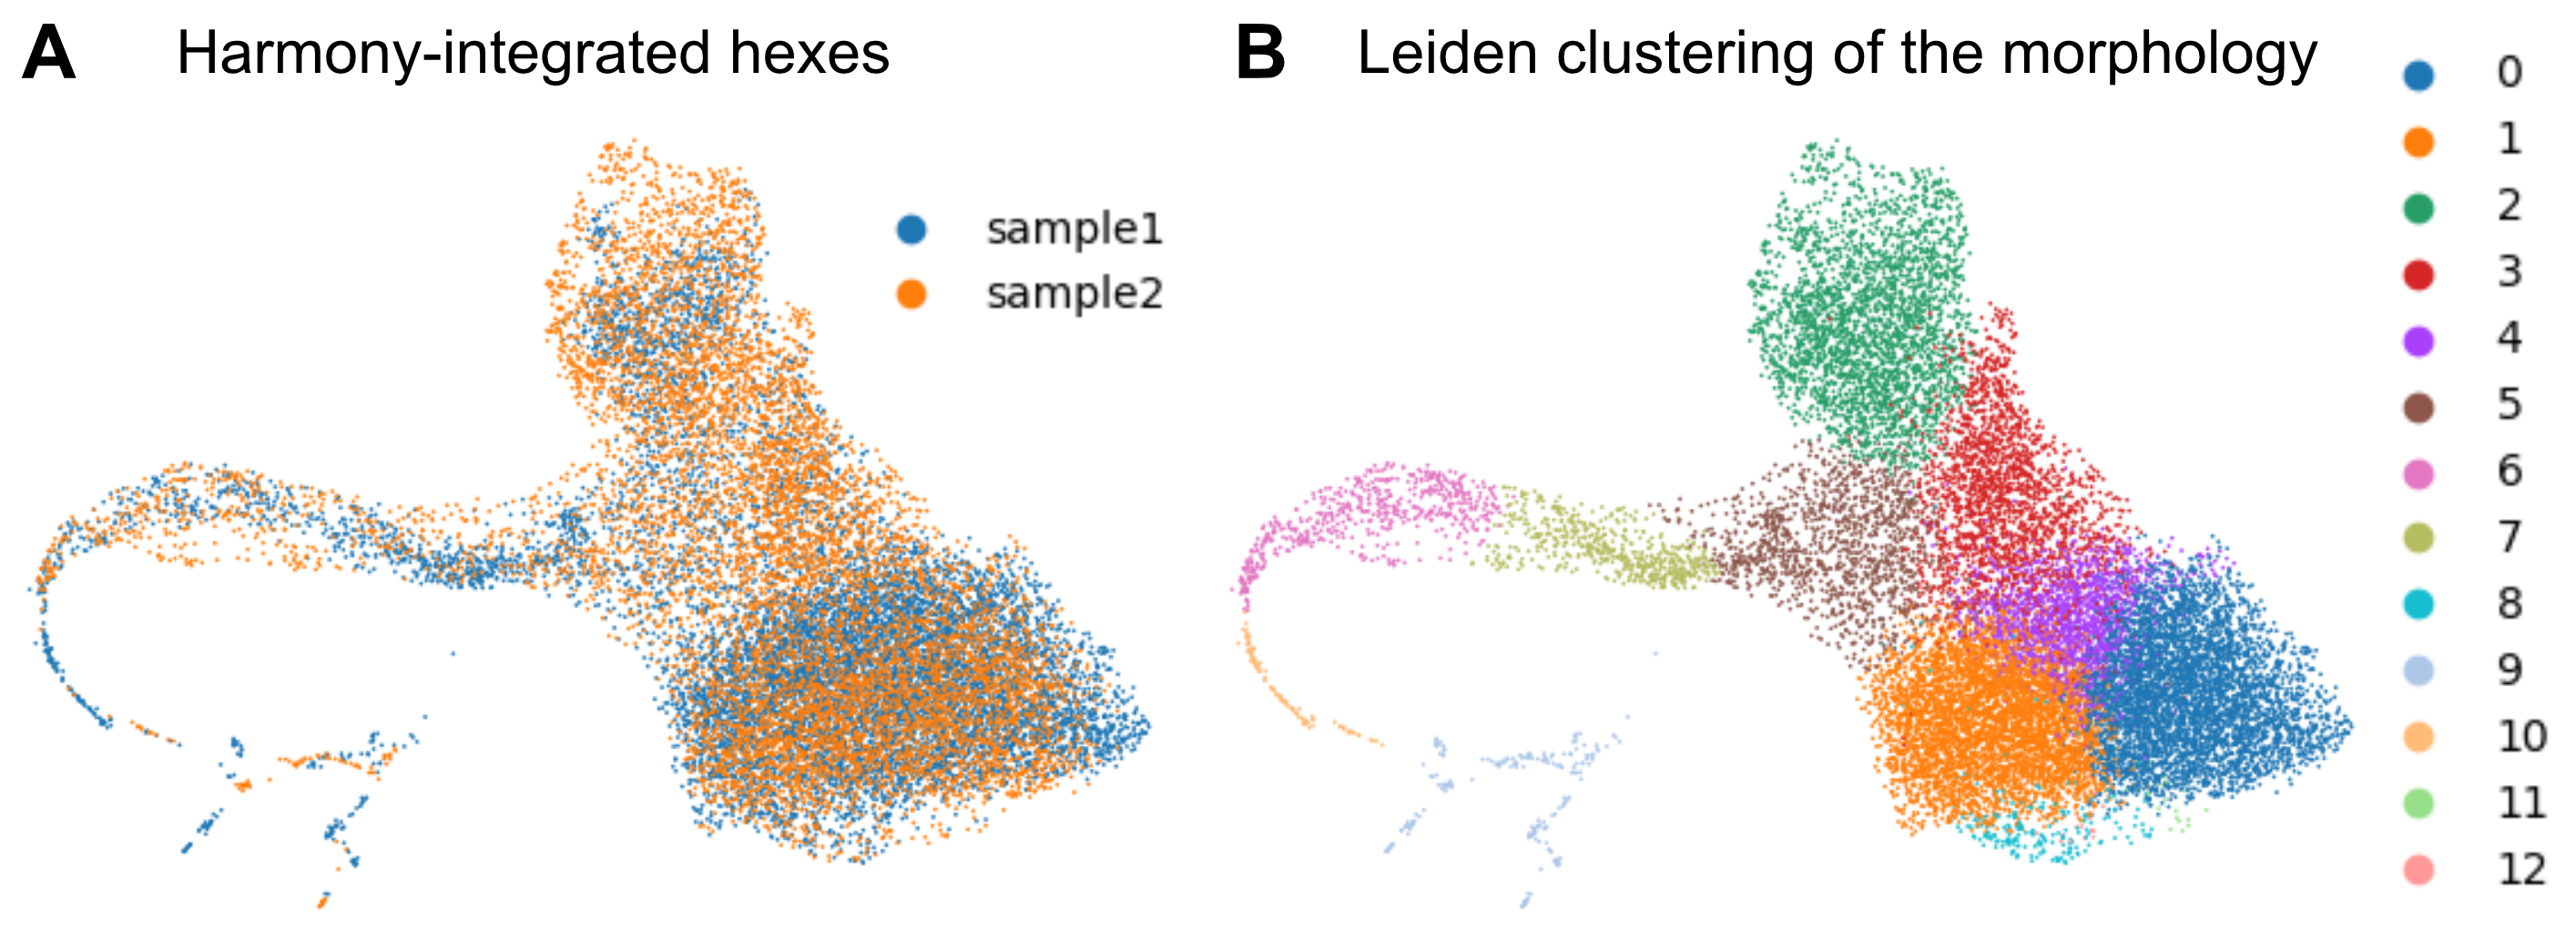
\includegraphics[width=.8\linewidth]{./figs/fig_S1_spatial_umap.png}
\caption{\label{fig:spatial_umap}{}UMAP projection of the processed morphology features. \textbf{Panel A.} Coloured by sample of origin, we see good mixing after the Harmony integration. \textbf{Panel B.} Coloured by Leiden clustering.}
\end{figure}

Due to the low cell count in Leiden cluster 10 for sample 2, as shown in Figure~\ref{fig:spatial_c10}B the cluster was excluded for some analysis steps.

\begin{figure}[htbp]
\centering
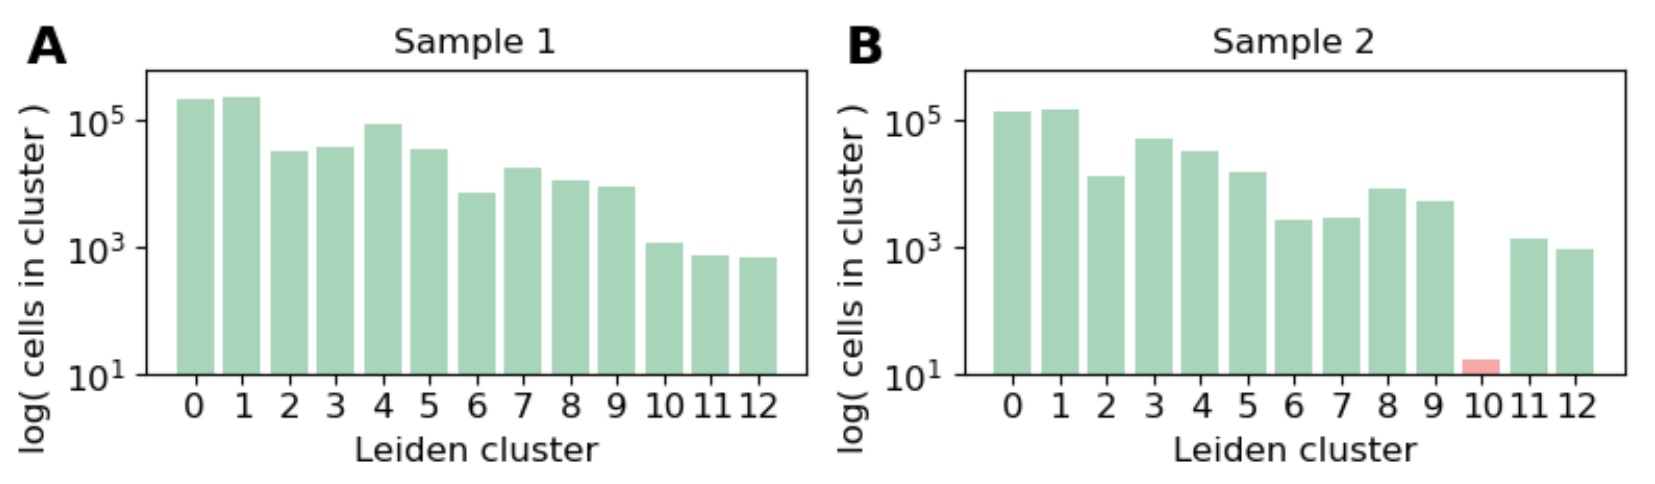
\includegraphics[width=.7\linewidth]{./figs/fig_S4_spatial_c10.png}
\caption{\label{fig:spatial_c10}{}Morphology reveals the composition of tumour subregions. \textbf{Panel A.} Spatial map of cell types inferred from transcriptomics. \textbf{Panel B.} Morphological subregions obtained by applying Leiden clustering to image-derived feature embeddings. \textbf{Panel C.} Bar chart showing, for each morphological cluster, the fraction of cells assigned to each cell type (colour legend as shown). The top left quarter of Panel A shows that the morphological approach worked to predict regions while the expression annotations did not.}
\end{figure}

\newpage

Then, the gene expression data from the Xenium experiment was used to annotate cell types for both samples. For every Leiden cluster, as defined by the Leiden clustering of the joint morphology features from both samples, the cells covered by the respective hexagons were extracted. Figure~\ref{fig:spatial_hne} shows the raw H\&E images, the distribution of cell types across these, and the hexagons coloured by their respective Leiden cluster. Of note is that the H\&E images both seemed to be partially corrupted, resulting in blacked-out sections. While the data contains cell segmentation masks for these sections, we filtered out hexagons overlaying these corrupted regions for the morphology featurization.

\begin{figure}[htbp]
\centering
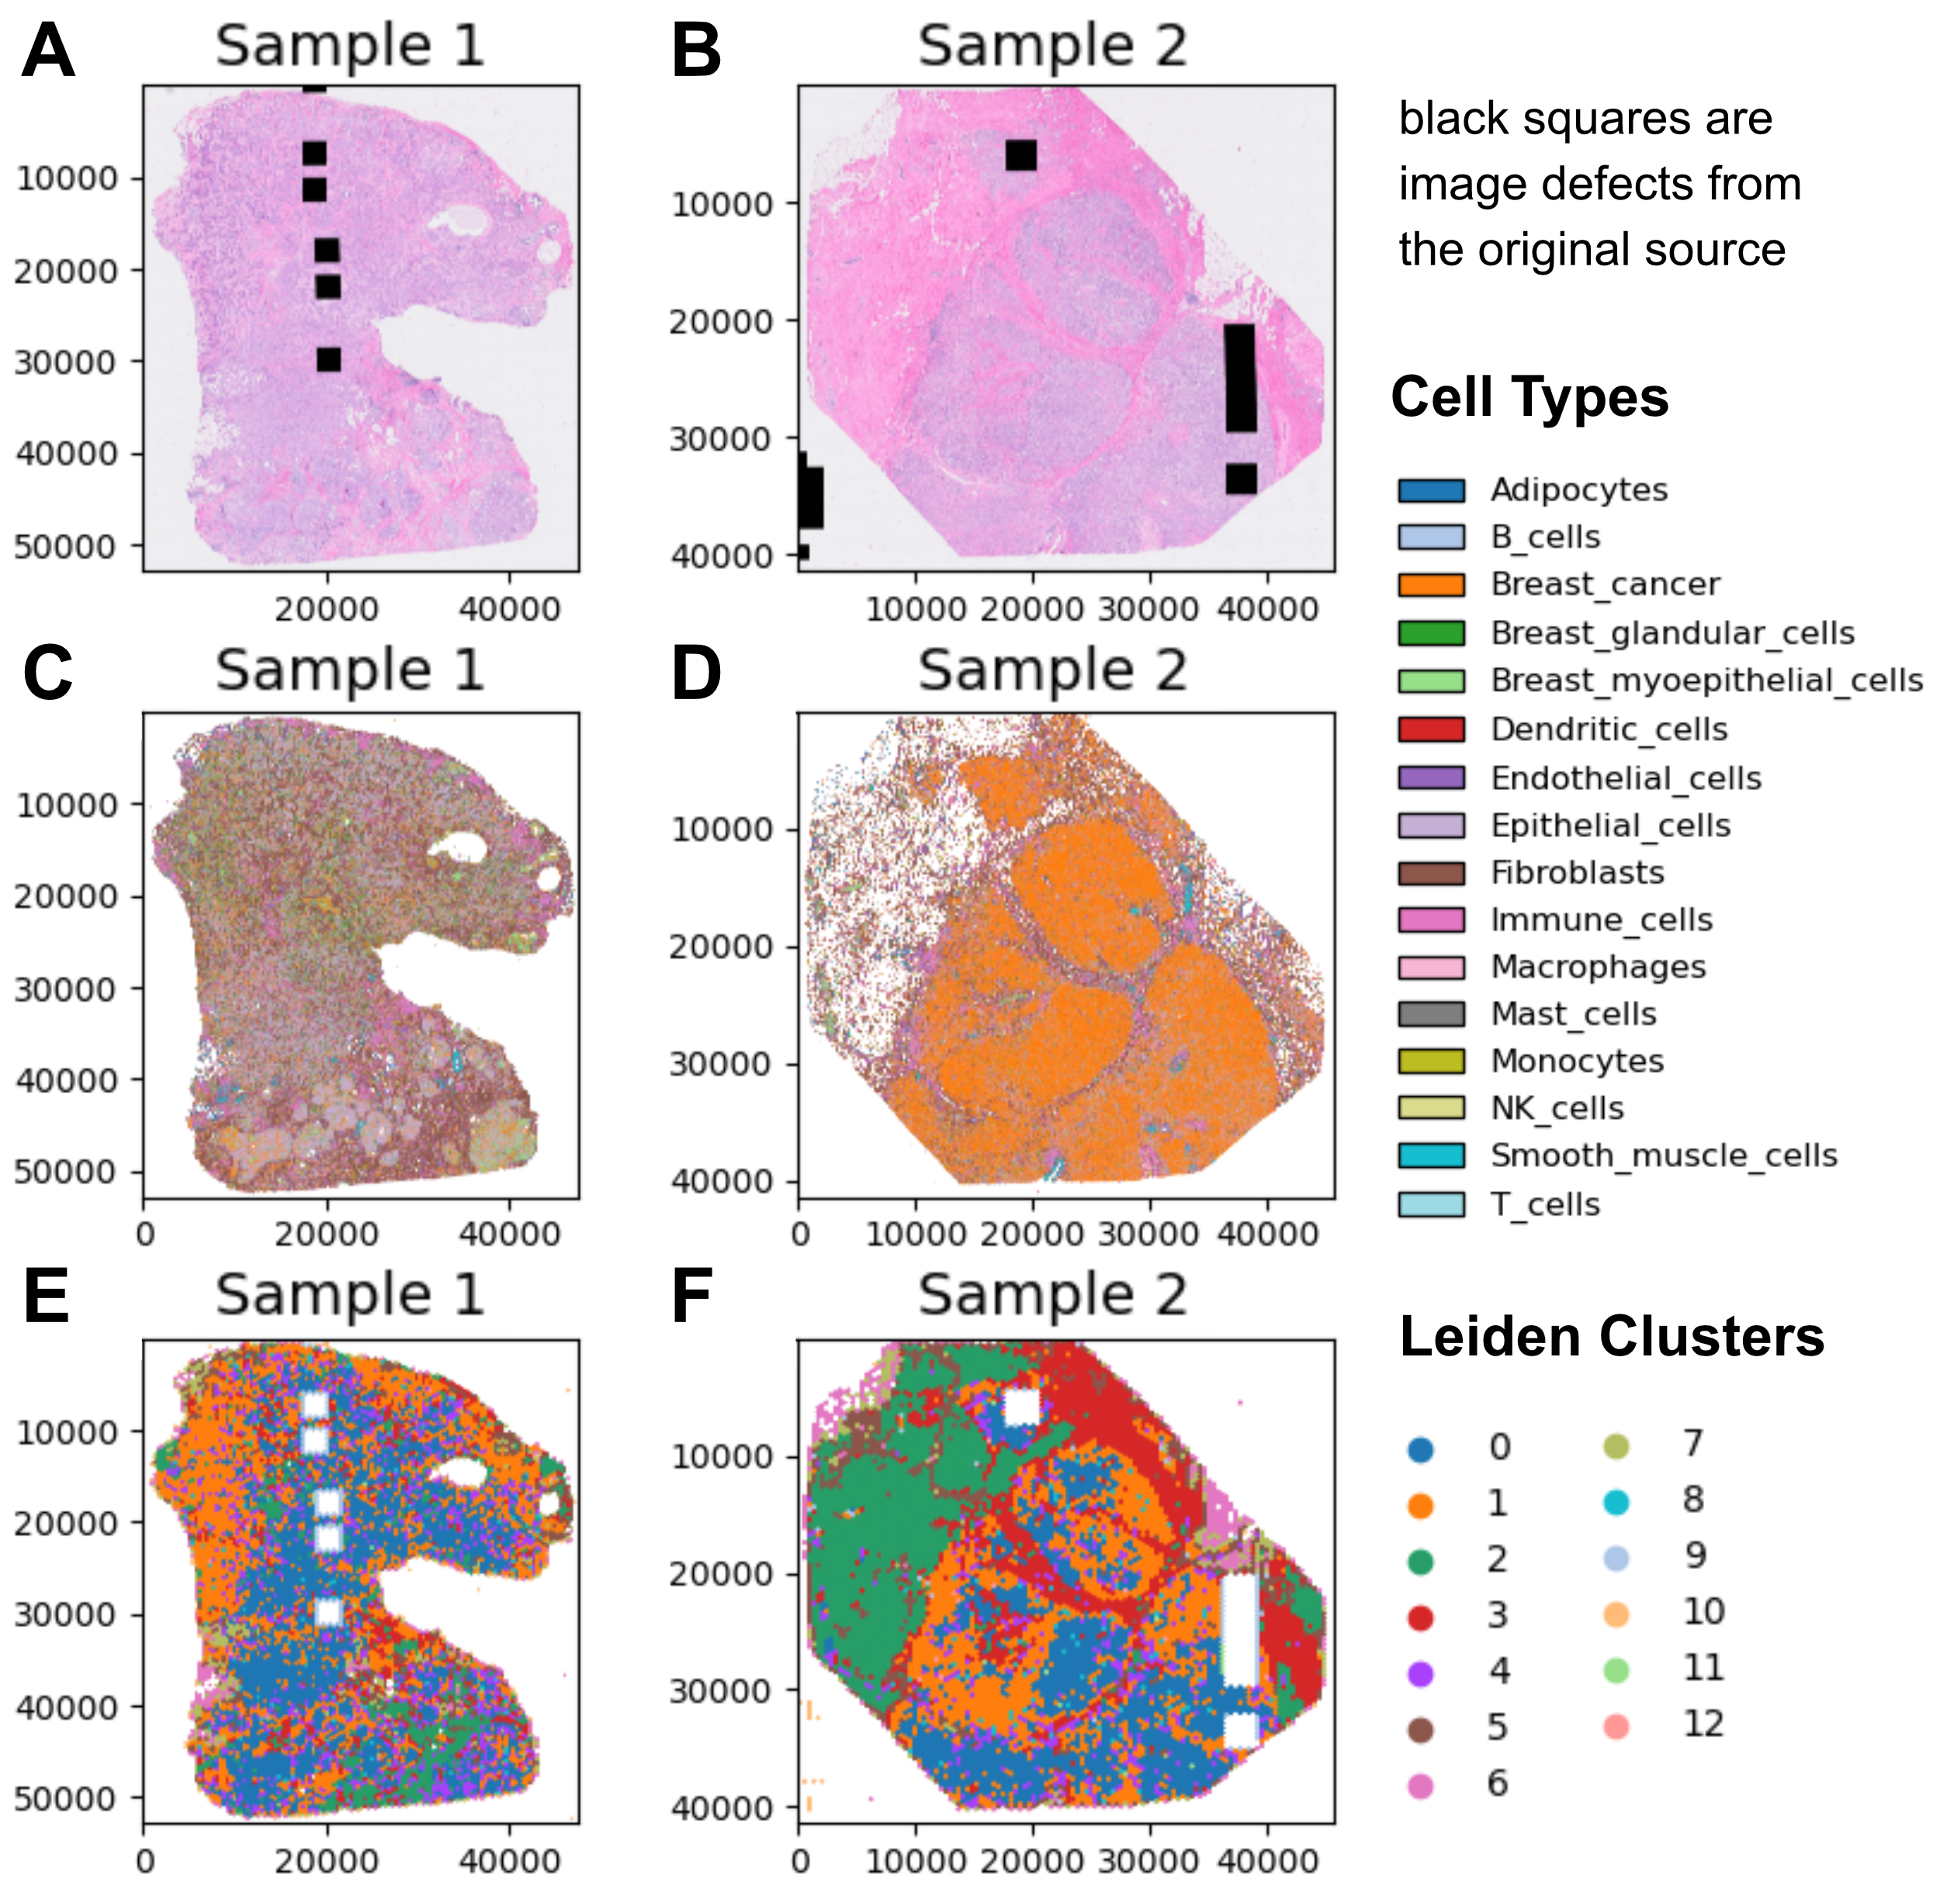
\includegraphics[width=.65\linewidth]{./figs/fig_S2_spatial_hne.png}
\caption{\label{fig:spatial_hne}{}Overview about the spatial distribution of cell types and morphology clusters. \textbf{Panel A and B.} H\&E images of both samples. \textbf{Panel C and D.} Cell segmentation masks colored by cell type. \textbf{Panel E and F.} Hexagons colored by their morphology Leiden cluster.}
\end{figure}

For every morphology Leiden cluster, we counted all cells whose centroids fell into the respective hexagons and calculated each cell type's share of the total cells per cluster. This data is shown in Figure~\ref{fig:spatial_composition}.

\begin{figure}[htbp!]
\centering
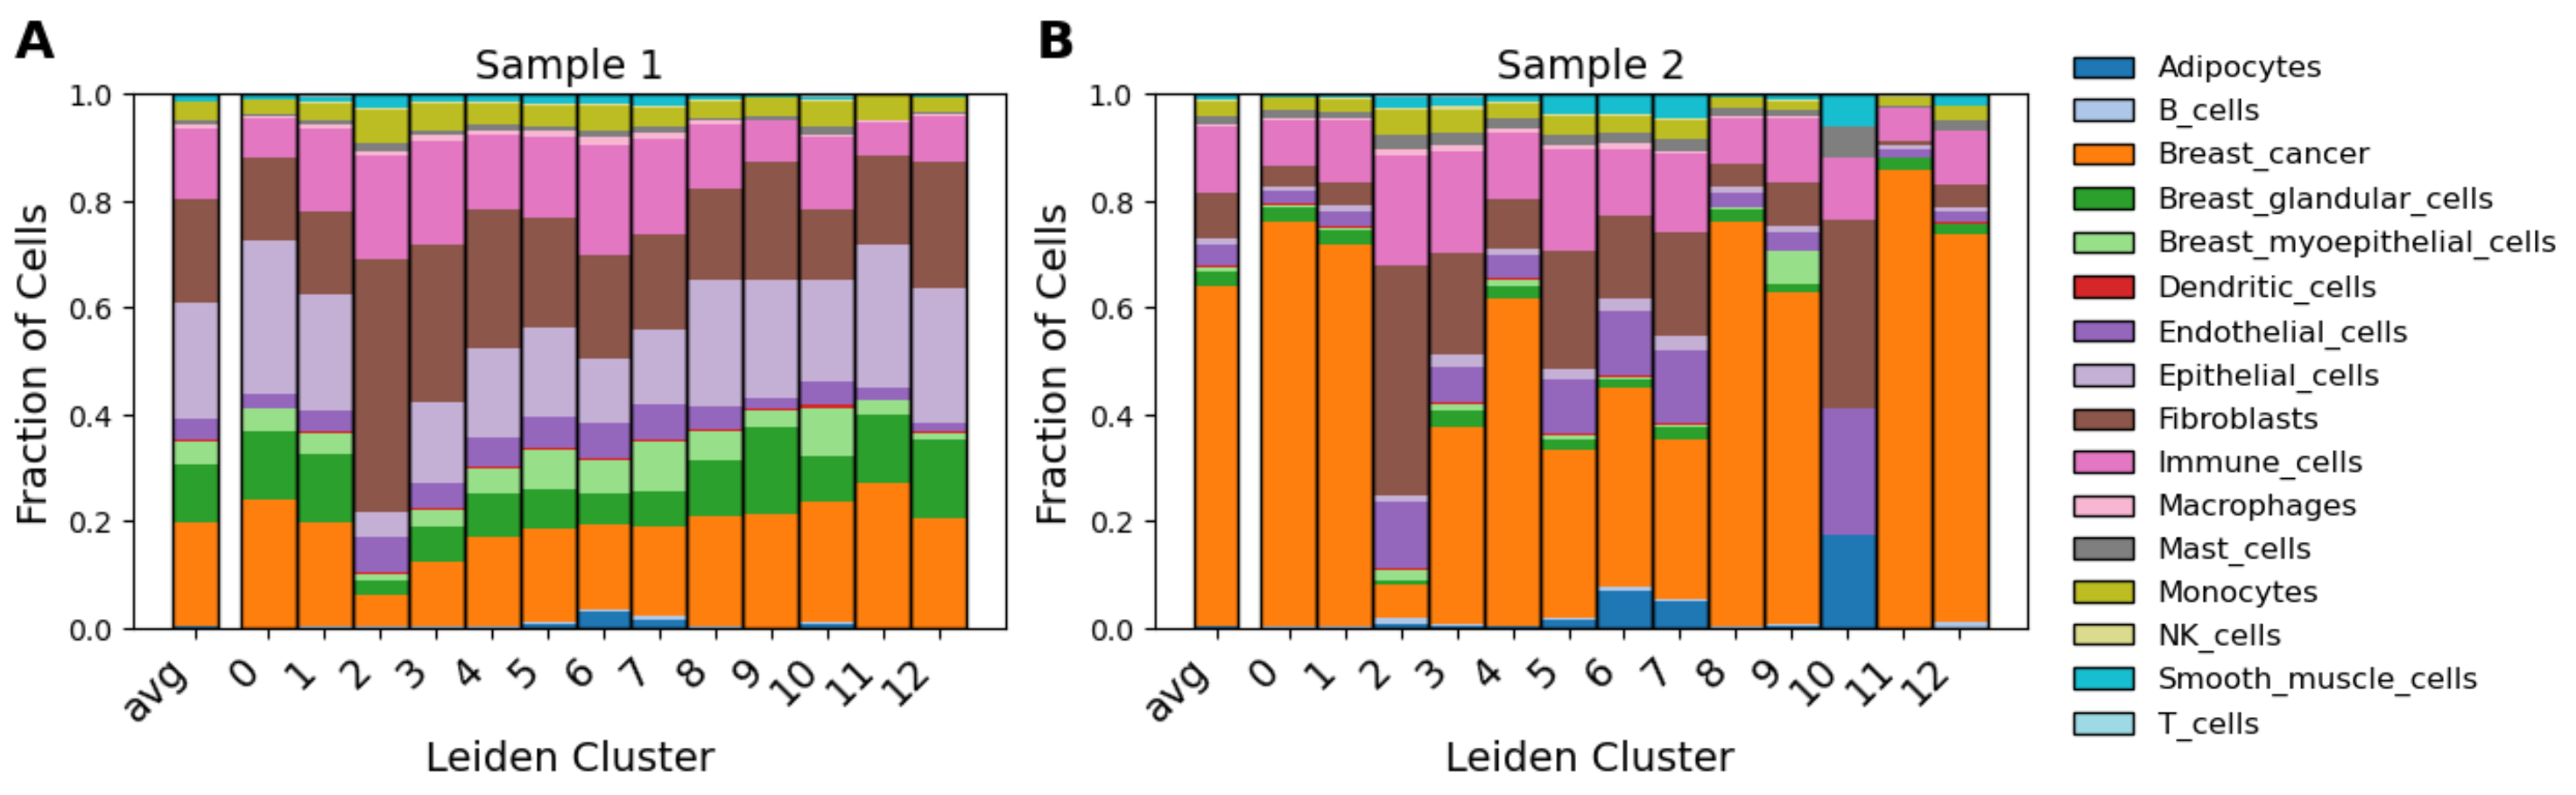
\includegraphics[width=.95\linewidth]{./figs/fig_S3_spatial_composition.png}
\caption{\label{fig:spatial_composition}{}Barplots showing the per-cluster cell type composition for both samples. Additionally, the average per sample is shown.}
\end{figure}

\newpage

Based on \citep{Wu2024-zp} we define an immune-hot signature comprising B~cells, dendritic~cells, NK~cells, and T~cells. For every Leiden cluster, we aggregated the respective cell type counts of this signature for both samples. These are shown in Figure~\ref{fig:spatial_immunehot}B and provide initial evidence for the difference in clusters 0 and 1, despite both being visually mixed as can be seen in Figure~\ref{fig:spatial_immunehot}A.

\begin{figure}[htbp!]
\centering
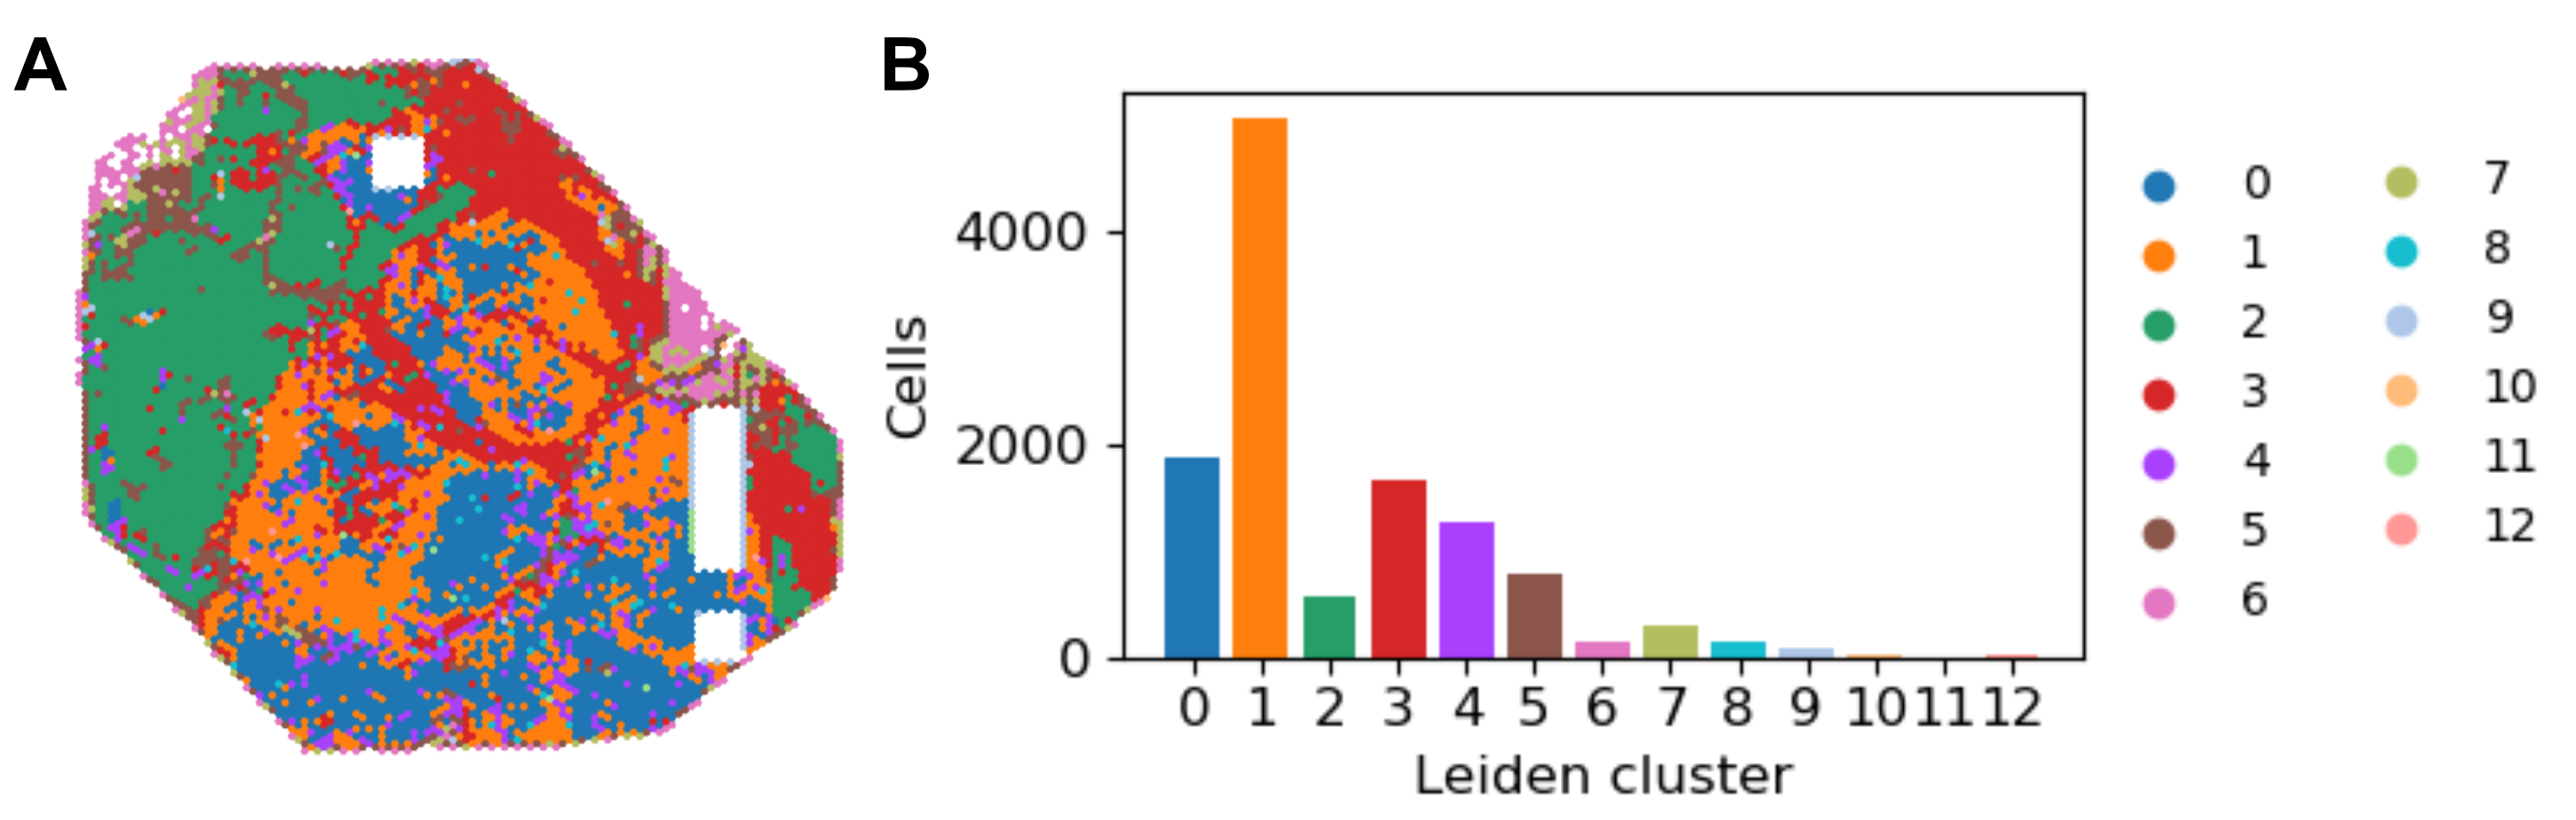
\includegraphics[width=.85\linewidth]{./figs/fig_S5_immunehot.png}
\caption{\label{fig:spatial_immunehot}{}Potential explanation of the differences between cluster~0 and cluster~1. \textbf{Panel A} Hexagons in sample~2 coloured by Leiden cluster. \textbf{Panel B} Cumulative counts of B~cells, dendritic~cells, NK~cells, and T~cells.}
\end{figure}


\bibliographystyle{icml2025}
\bibliography{bibliography}

\end{document}
